\documentclass[a4paper,11pt]{article}

\usepackage{mathtools}
\usepackage{amssymb}
\usepackage{hyperref}
\usepackage[cm]{fullpage}
\usepackage{fancyhdr}
\usepackage[ddmmyyyy]{datetime} 
\usepackage[]{graphicx}
\usepackage{hhline}
\usepackage{listings}
\usepackage{enumitem}
\usepackage{todonotes}

\graphicspath{{figures}}

% Settings for listings package
\definecolor{mygreen}{rgb}{0,0.6,0}
\definecolor{mygray}{rgb}{0.5,0.5,0.5}
\definecolor{mymauve}{rgb}{0.58,0,0.82}
\definecolor{altblue}{rgb}{0.0,0.6,1.0}
\definecolor{lstbg}{gray}{0.9}

\lstset{
  backgroundcolor=\color{lstbg},
  % choose the background color; you must add \usepackage{color} or \usepackage{xcolor}
  basicstyle=\footnotesize\ttfamily,
  % the size of the fonts that are used for the code
  breakatwhitespace=true,
  % sets if automatic breaks should only happen at whitespace
  breaklines=true,
  % sets automatic line breaking
  captionpos=b,
  % sets the caption-position to bottom
  commentstyle=\color{mygreen},
  % comment style
  deletekeywords={},
  % if you want to delete keywords from the given language
  escapeinside={\#*}{*},
  % if you want to add LaTeX within your code
  extendedchars=true,
  % lets you use non-ASCII characters; for 8-bits encodings only, does not work with UTF-8
  frame=single,
  % adds a frame around the code
  keepspaces=true,
  % keeps spaces in text, useful for keeping indentation of code (possibly needs columns=flexible)
  keywordstyle=\color{blue},
  % keyword style
  %language=c++,
  % the language of the code
  otherkeywords={},
  % if you want to add more keywords to the set
  numbers=left,
  % where to put the line-numbers; possible values are (none, left, right)
  numbersep=5pt,
  % how far the line-numbers are from the code
  numberstyle=\tiny\color{mygray},
  % the style that is used for the line-numbers
  rulecolor=\color{black},
  % if not set, the frame-color may be changed on line-breaks within not-black text (e.g. comments (green here))
  showspaces=false,
  % show spaces everywhere adding particular underscores; it overrides 'showstringspaces'
  showstringspaces=false,
  % underline spaces within strings only
  showtabs=false,
  % show tabs within strings adding particular underscores
  stepnumber=1,
  % the step between two line-numbers. If it's 1, each line will be numbered
  stringstyle=\color{mymauve},
  % string literal style
  tabsize=4,
  % sets default tabsize to 4 spaces
  title=\lstname
  % show the filename of files included with \lstinputlisting; also try caption instead of title
}

\hypersetup{
	colorlinks=true,
	urlcolor=blue
}

\title{\textsc{Scalable and robust Firedrake deployment on ARCHER2 and beyond}\\
\Large ARCHER2-eCSE04-5}
\author{Jack Betteridge}
\date{30/4/2022}
% PI: Dr David A Ham (Imperial College) 

\pagestyle{fancy}
\setlength{\headheight}{15pt}
\setlength{\headsep}{5pt}
\lhead{ \fancyplain{}{} }
\rhead{ \fancyplain{}{Jack Betteridge} }
%\lhead[\footnotesize\nouppercase{\leftmark}]{}
%\rhead[]{\footnotesize\nouppercase{\rightmark}}

\renewcommand{\footrulewidth}{0.4pt}
\cfoot[-- \thepage\ --]{-- \thepage\ --}

\begin{document}
%\maketitle


%%%%%%%%%%%%%%%%%%%%%%%%%
\begin{center}\huge\textsc{Scalable and robust Firedrake deployment on ARCHER2 and beyond}\end{center}
\section*{}
\label{sec:intro}
%%%%%%%%%%%%%%%%%%%%%%%%%
% A summary of the science that will benefit from the eCSE. Describe any potential impact. Why is this work of value to society?
% Provide an overview of the work carried out. What has been done to the application code? What has been achieved?
% A brief summary of the application codes involved. 
% Include any relevant publications
% If at all possible, please provide an image.
Spack (\url{https://spack.io/}) is a package manager specifically designed for HPC users for installing popular software packages.
We have created a package for Spack to install Firedrake (\url{https://firedrakeproject.org/}), an automated system for the solution of partial differential equations using the finite element method (FEM) and sophisticated code generation.
Through this work we have developed a workflow for using Spack on ARCHER2, which can be utilised by any HPC user.
Packages within Spack have been improved, updated and contributed back to the Spack project, which make packages easier to install on ARCHER2.
This work will benefit all users of ARCHER2 who wish to install packages not provided already on the system.
In addition, many of Firedrake's other dependencies have had Spack packages developed or modified to allow for the easy installation of Firedrake.
Furthermore, we have created Spack packages for some applications that themselves depend on Firedrake, so that users of these tools can install the software and immediately start doing science, these include (amongst others):
\begin{itemize}[topsep=2pt, partopsep=0pt, itemsep=1pt, parsep=1pt]
	\item \textbf{Gusto} a Firedrake dynamical core toolkit for weather modelling.
	\item \textbf{Thetis} an unstructured grid coastal ocean model.
	\item \textbf{Icepack} a package for solving the equations of motion of glacier flow using Firedrake.
\end{itemize}
The availability of a Spack package will save huge amounts of person time performing bespoke Firedrake installations and even allows for system level installations, where Spack is centrally supported.

\begin{figure}[htp]
	\centering
	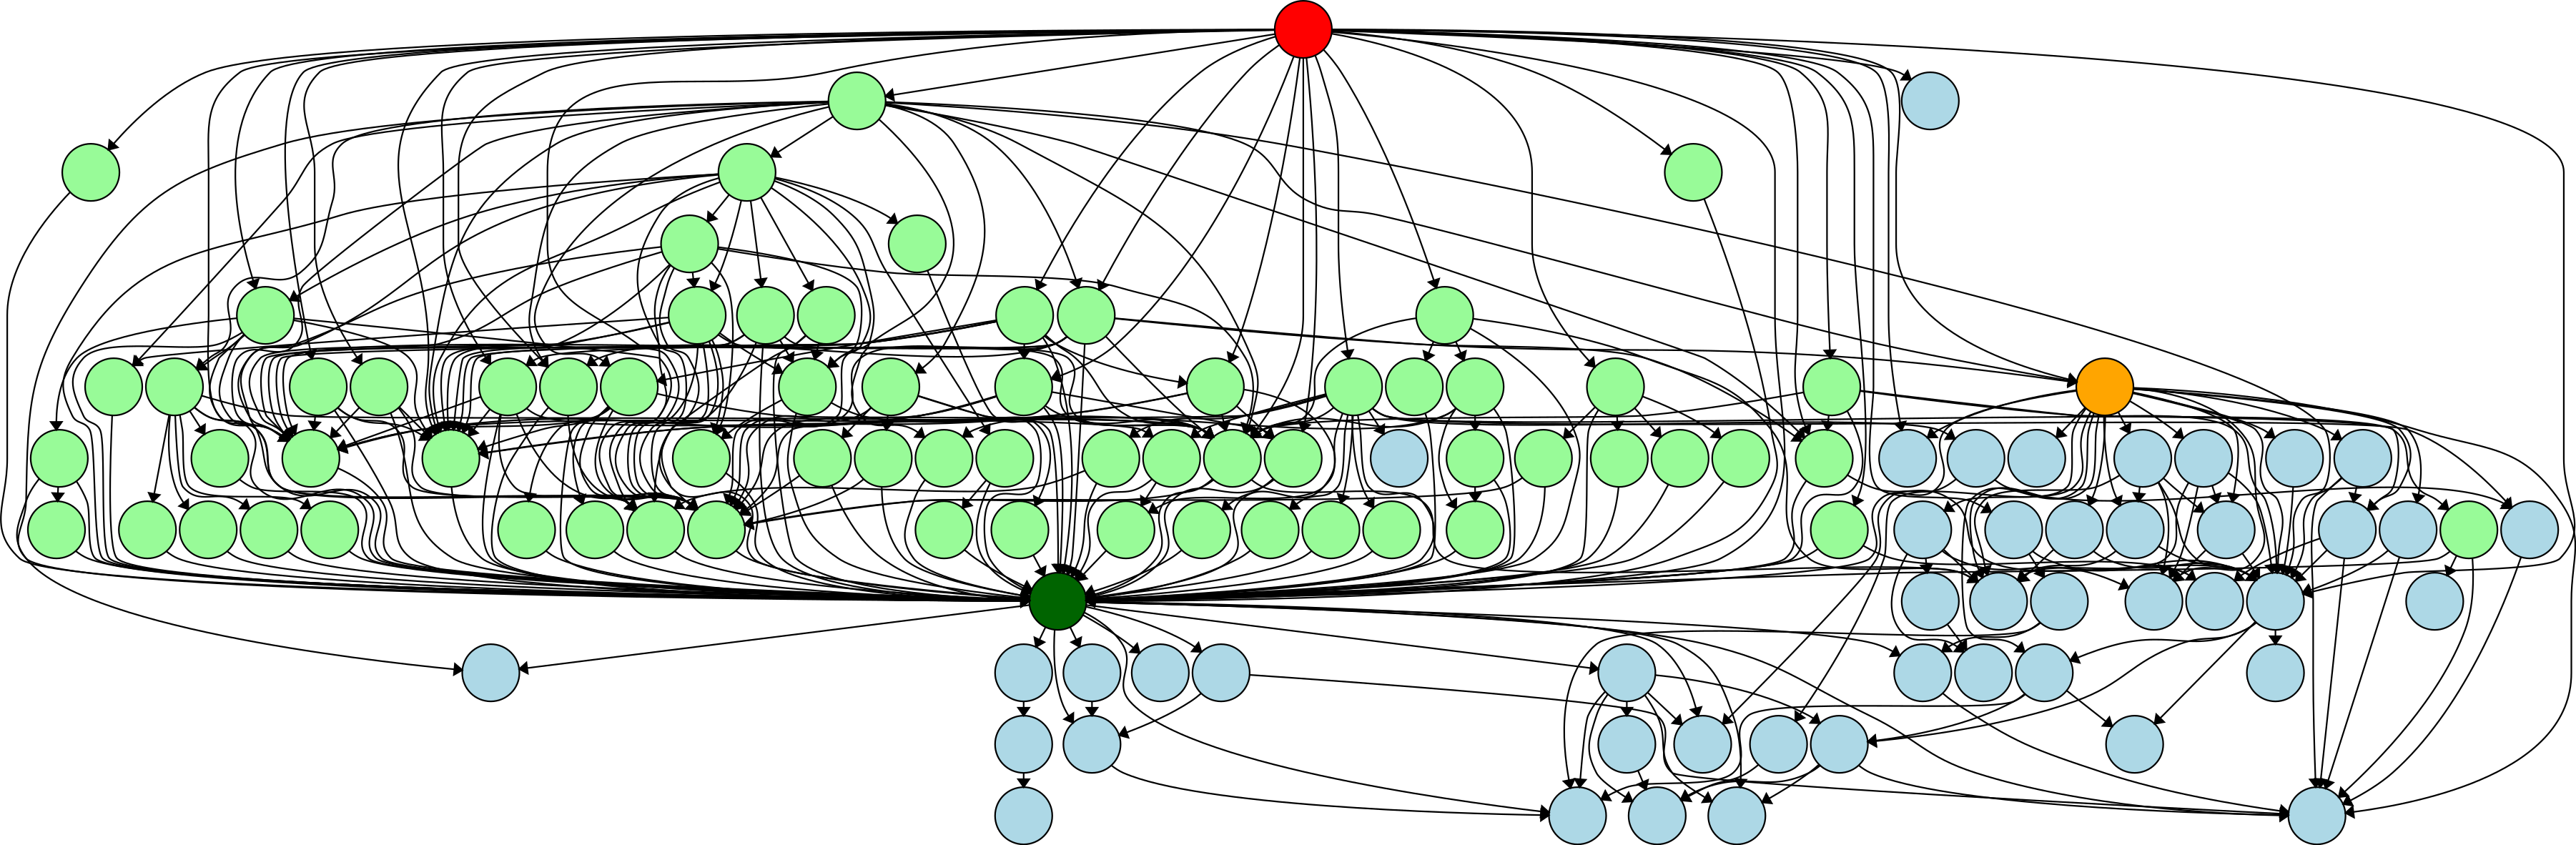
\includegraphics[width=\textwidth]{firedrake_deps.png}
	\caption{A directed graph showing the complexity of Firedrake's dependencies. Firedrake is highlighted at the top in red, Python as dark green and Python packages as light green. The orange circle is PETSc and all remaining pale blue circles are compiled dependencies. Generated by the command:\\ \texttt{spack graph -d py-firedrake \%gcc \^{}mpich \^{}openblas \textgreater{} py-firedrake.dot}}
	\label{fig:fddeps}
\end{figure}

Docker is a popular container environment for users on their own local machines, but is not suitable for HPC environments as it allows for privilege escalation.
Singularity is installed as a module on ARCHER2, but it is not possible for users to build their own images from scratch.
We have developed a Singularity image for Firedrake based on the Firedrake Docker images so that end users who do not wish to modify the Firedrake source can have a zero installation route to running their Firedrake scripts.
These singularity images have been tested to make sure they are suitable for use on ARCHER2 and remain performant.

PETSc is a key Firedrake dependency and provides a lot of the solvers used for simulations.
During the course of the eCSE we identified a parallel deadlock bug, which occurs when Python tries to clean up memory belonging to petsc4py on some ranks, but not others.
The frequency of this bug occurring increases with then number of MPI ranks, meaning it is more prevalent when running on large HPC facilities, like ARCHER2.
We have designed an algorithm for the safe parallel collection of distributed Python objects, like those found in petsc4py.
An implementation of this algorithm has been contributed to PETSc to prevent deadlock occurring when using PETSc in combination with other memory managed languages, such as Python or Julia.


\end{document}